\providecommand{\main}{../../../..}
\documentclass[\main/dresen_thesis.tex]{subfiles}
\begin{document}
  \begin{figure}[tb]
    \centering
    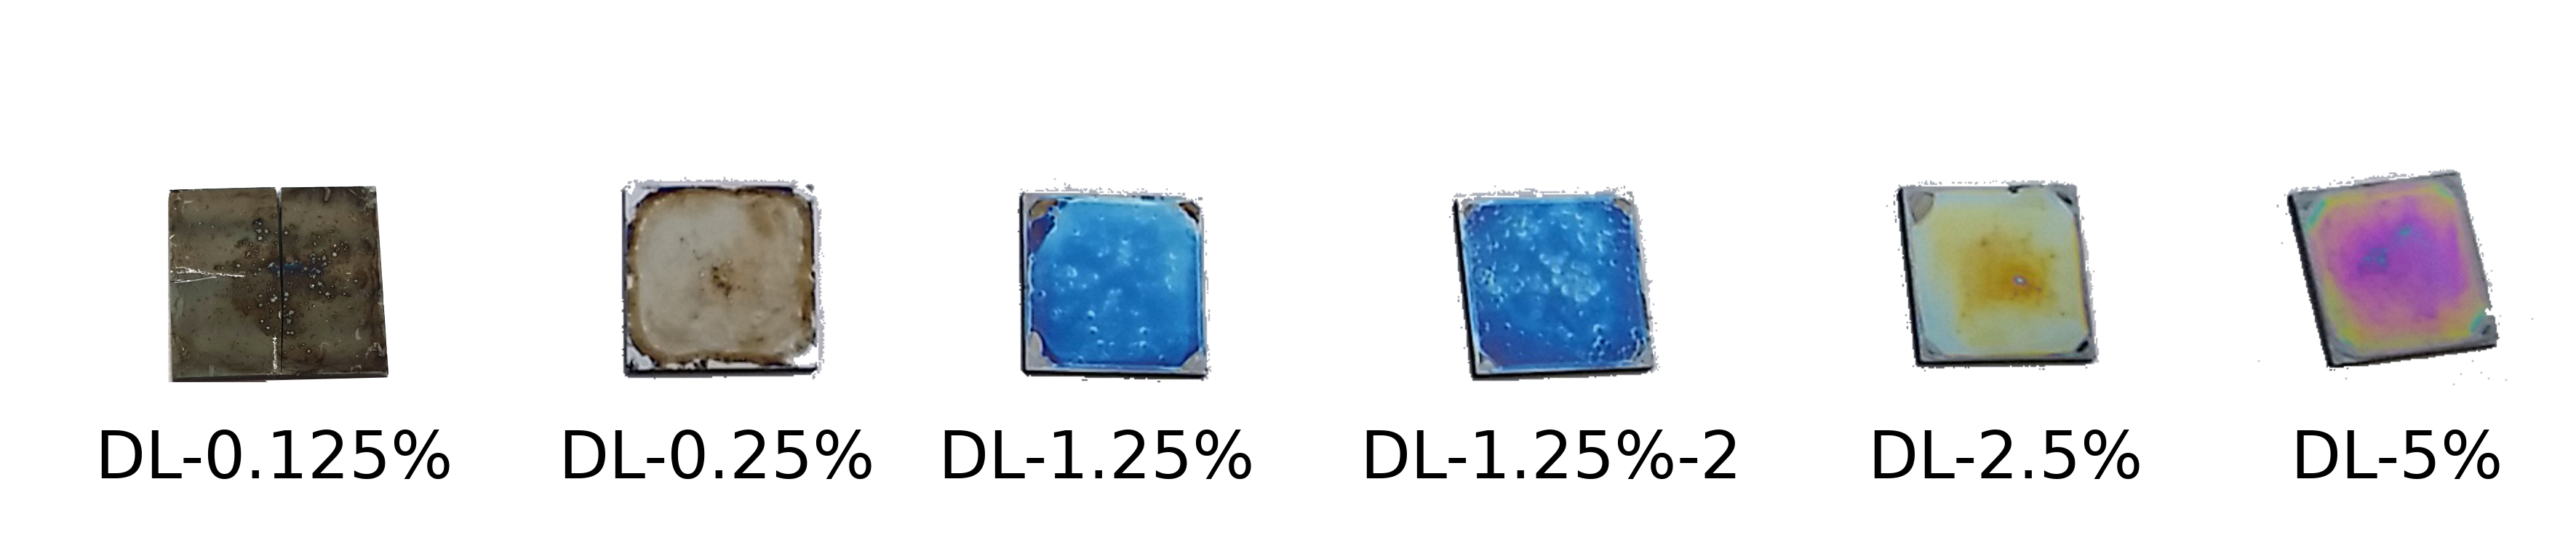
\includegraphics{doubleLayer_wafers}
    \caption{\label{fig:doubleLayers:preparation:waferImage}Image of prepared wafers}
  \end{figure}

  The drop casting procedure described in \refsec{sec:monolayers:preparation} can be extended to prepare double layers with intermediate spacer layers of variable thickness.
  For this purpose, in a first step six monolayers are prepared according to the aforementioned protocol.
  To add a PMMA layer on top, commercially obtained PMMA is dissolved with a volume concentration of $5 \%$ in a first step in ethyl acetate (EtOAc) by heating $1.1809 \unit{mg}$ PMMA in $25 \unit{mL}$ EtOAc at $40 \unit{^\circ C}$ for two hours until a clear solution is obtained.
  Four dilutions from the PMMA stock solution are prepared by adding additional EtOAc to the stock solution in separate beakers.

  On the prepared monolayers, $80 \unit{\textmu L}$ of the dispersions with PMMA concentrations tabulated in \reftab{tab:doubleLayers:preparation:samples} are dropped equally distributed on the surface of the sample and spin coated at $33 \unit{rps}$ for $60 \unit{s}$.
  The spin coating process is initialized with a $10 \unit{s}$ ramp up procedure at $3 \unit{rps}$ to ensure a homogeneous distribution of the PMMA dispersion.
  The sample is then dried in an oven at $80 ^\circ C$ for $2 \unit{h}$ and after cooling back down to room temperature, a second monolayer is drop casted on top in the same procedure as the first one was done.
  The finally obtained sample is not washed by non-polar solvent as to avoid dissolving the intermediate PMMA thickness, which is only weakly protected by the upper nanoparticle layer.

  \begin{table}[!htbp]
    \centering
    \caption{\label{tab:doubleLayers:preparation:samples}Samples studied in this chapter.}
    \begin{tabular}{ l | l | l | l}
      \textbf{Sample}  & $c_V^\mathrm{PMMA}$ & color & characterization\\
      \hline
      DL-0.125\%    & $0.125$ & ?               & SEM, XRR, PNR, VSM\\
      DL-0.25\%     & $0.25$ & brown            & SEM, XRR, PNR, VSM\\
      DL-1.25\%     & $1.25$ & blue             & SEM, XRR, PNR, VSM\\
      DL-1.25-2\%   & $1.25$ & blue             & SEM, XRR\\
      DL-2.5\%      & $2.50$ & light blue/yellow& SEM, XRR, PNR, VSM\\
      DL-5\%        & $5.00$ & purple           & SEM, XRR, VSM\\
      \hline
    \end{tabular}
  \end{table}

  % DL-0.50\%     & $0.50$ & brown            & SEM \\
  % DL-5\%-2      & $5.00$ & green            & SEM \\

\end{document}